% TikZ schematic: Adaptive Pipeline Flow
% Standalone version - compile with pdflatex
\documentclass[border=10pt]{standalone}
\usepackage{tikz}
\usepackage{xcolor}
\usetikzlibrary{shapes,arrows,positioning,calc,decorations.pathreplacing,patterns,fit,backgrounds}

\definecolor{inputblue}{RGB}{31,119,180}
\definecolor{fftgreen}{RGB}{44,160,44}
\definecolor{featorange}{RGB}{255,127,14}
\definecolor{arrowgray}{RGB}{100,100,100}

\begin{document}
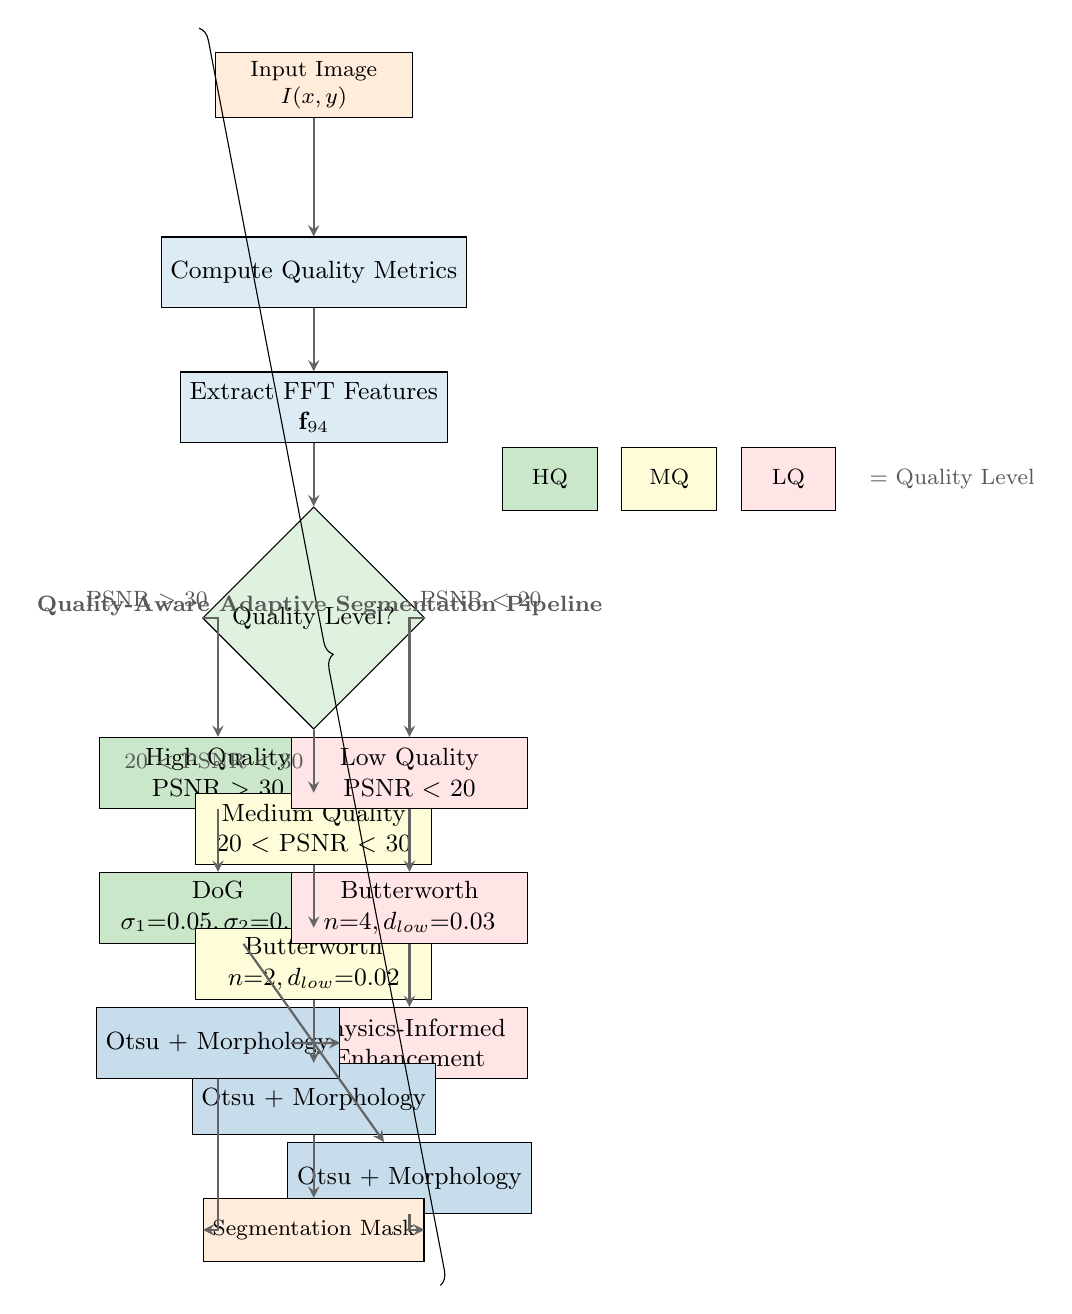
\begin{tikzpicture}[
 node distance=1.5cm and 2cm,
 block/.style={rectangle, draw, fill=inputblue!15, minimum width=3cm, minimum height=0.9cm, align=center, font=\small},
 decision/.style={diamond, draw, fill=fftgreen!15, minimum width=2.5cm, minimum height=1cm, align=center, font=\small},
 data/.style={rectangle, draw, fill=featorange!15, minimum width=2.5cm, minimum height=0.8cm, align=center, font=\footnotesize},
 arrow/.style={->, >=stealth, thick, color=arrowgray},
 label/.style={font=\footnotesize, color=gray!70!black}
]

% Row 1: Input
\node[data] (input) {Input Image\\$I(x,y)$}; 

% Row 2: Quality Assessment
\node[block, below=of input] (quality) {Compute Quality Metrics}; 
\node[block, below=0.8cm of quality] (features) {Extract FFT Features\\$\mathbf{f}_{94}$}; 

% Row 3: Decision
\node[decision, below=0.8cm of features] (decide) {Quality Level?}; 

% Row 4: Branches
\node[block, below left=0.8cm and -1cm of decide, fill=fftgreen!25] (hq) {High Quality\\PSNR $>$ 30}; 
\node[block, below=0.8cm of decide, fill=yellow!15] (mq) {Medium Quality\\20 $<$ PSNR $<$ 30}; 
\node[block, below right=0.8cm and -1cm of decide, fill=red!10] (lq) {Low Quality\\PSNR $<$ 20}; 

% Row 5: Filter Selection
\node[block, below=0.8cm of hq, fill=fftgreen!25] (hq_filter) {DoG\\$\sigma_1{=}0.05, \sigma_2{=}0.20$}; 
\node[block, below=0.8cm of mq, fill=yellow!15] (mq_filter) {Butterworth\\$n{=}2, d_{low}{=}0.02$}; 
\node[block, below=0.8cm of lq, fill=red!10] (lq_filter) {Butterworth\\$n{=}4, d_{low}{=}0.03$}; 

% Row 6: Enhancement (for LQ only)
\node[block, below=0.8cm of lq_filter, fill=red!10] (enhance) {Physics-Informed\\Enhancement}; 

% Row 7: Segmentation
\node[block, below=0.8cm of enhance, fill=inputblue!25] (seg_hq) {Otsu + Morphology}; 
\node[block, below=0.8cm of mq_filter, fill=inputblue!25] (seg_mq) {Otsu + Morphology}; 
\node[block, below=0.8cm of hq_filter, fill=inputblue!25] (seg_lq) {Otsu + Morphology}; 

% Row 8: Output
\node[data, below=0.8cm of seg_mq] (output) {Segmentation Mask}; 

% Arrows
\draw[arrow] (input) -- (quality);
\draw[arrow] (quality) -- (features);
\draw[arrow] (features) -- (decide);

\draw[arrow] (decide) -| node[above left, label] {PSNR $>$ 30} (hq);
\draw[arrow] (decide) -- node[left, label] {20 $<$ PSNR $<$ 30} (mq);
\draw[arrow] (decide) -| node[above right, label] {PSNR $<$ 20} (lq);

\draw[arrow] (hq) -- (hq_filter);
\draw[arrow] (mq) -- (mq_filter);
\draw[arrow] (lq) -- (lq_filter);
\draw[arrow] (lq_filter) -- (enhance);
\draw[arrow] (enhance) -- (seg_lq);
\draw[arrow] (mq_filter) -- (seg_mq);
\draw[arrow] (hq_filter) -- (seg_hq);

\draw[arrow] (seg_hq) |- (output);
\draw[arrow] (seg_mq) -- (output);
\draw[arrow] (seg_lq) |- (output);

% Brace
\draw[decorate, decoration={brace, amplitude=5pt}]
 ($(input.north west)+(-0.2,0.3)$) -- ($(output.south east)+(0.2,-0.3)$)
 node[midway, above=0.4cm, label] {\textbf{Quality-Aware Adaptive Segmentation Pipeline}};

% Legend
\node[data, fill=fftgreen!25, minimum width=1.2cm] (leg1) at (3,-5) {HQ}; 
\node[data, fill=yellow!15, minimum width=1.2cm, right=0.3cm of leg1] (leg2) {MQ}; 
\node[data, fill=red!10, minimum width=1.2cm, right=0.3cm of leg2] (leg3) {LQ}; 
\node[label, right=0.3cm of leg3] {= Quality Level};

\end{tikzpicture}
\end{document}
